\documentclass[10pt]{beamer}

\usetheme{default}

\usepackage[utf8]{inputenc}
\usepackage[russian]{babel}
\usepackage[OT1]{fontenc}
\usepackage{amsmath}
\usepackage{amsfonts}
\usepackage{amssymb}
\usepackage{graphicx}
\usepackage{etoolbox}
\usepackage{caption}
\usepackage{subcaption}
\usepackage{pifont}
\usepackage{xcolor}
\usepackage{framed}
\definecolor{shadecolor}{cmyk}{0,0,0,1}
\usepackage{multirow}

\usepackage{listings}

\lstset{
	backgroundcolor=\color{lightgray},
	commentstyle=\color{blue},
	frame=single
	breakatwhitespace, 
	language=python, 
	columns=fullflexible, 
	keepspaces, 
	breaklines, 
	tabsize=3, 
	showstringspaces=false, 
	extendedchars=true,
	numbers=left
}

\makeatletter

\setbeamercolor{title}{fg=white}
\setbeamercolor{frametitle}{fg=black}
\setbeamerfont*{title}{family=\sffamily,size=\LARGE}

\setbeamerfont{page number in head/foot}{size=\scriptsize}
\setbeamertemplate{footline}[frame number]
\let\otp\titlepage
\renewcommand{\titlepage}{\otp\addtocounter{framenumber}{-1}}

\setbeamertemplate{background canvas}{%
	\ifnumequal{\c@framenumber}{0}{%
      
\includegraphics[width=\paperwidth,height=\paperheight]{images/cover.png}
   }{%
      \ifnumequal{\c@framenumber}{\inserttotalframenumber}{
         
\includegraphics[width=\paperwidth,height=\paperheight]{images/back.png}
      }{%
         % Other frames
      }%
   }%
}

\makeatother

\beamertemplatenavigationsymbolsempty

\author{Николай Анохин}
\title{\newline \newline \newline Лекция 6 \\ Задача классификации}

\begin{document}

\begin{frame}[plain]
\titlepage
\end{frame}

\begin{frame}{План занятия}
\tableofcontents
\end{frame}

% ========================================
\section{Задачи классификации и регрессии}
% ========================================

\begin{frame}{}

\begin{center}
\Large Задачи классификации и регрессии
\end{center}

\end{frame}

\begin{frame}{Классификация: интуиция}

\begin{block}{Задача}
Разработать алгоритм, позволяющий определить класс произвольного объекта из некоторго множества
\begin{itemize}
\item Дана {\it обучающая выборка}, в которой для каждого объекта известен класс
\end{itemize}
\end{block} 

\begin{center}
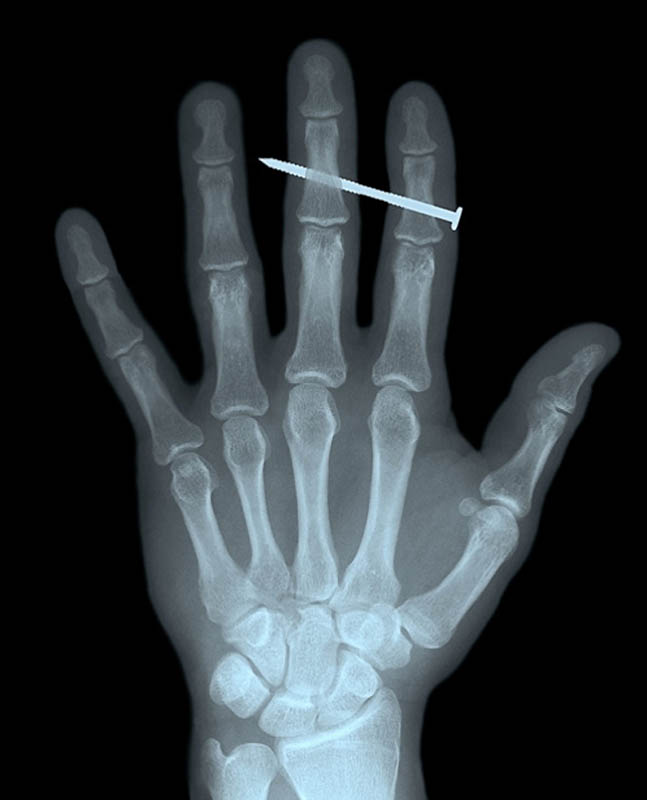
\includegraphics[scale=0.15]{images/xray.jpg}
\end{center}

\end{frame}

\begin{frame}{Регрессия: интуиция}

\begin{block}{Задача}
Разработать алгоритм, позволяющий предсказать числовую характеристику произвольного объекта из некоторого множества
\begin{itemize}
\item Дана {\it обучающая выборка}, в которой для каждого объекта известно значение числовой характеристики
\end{itemize}
\end{block}

\begin{center}
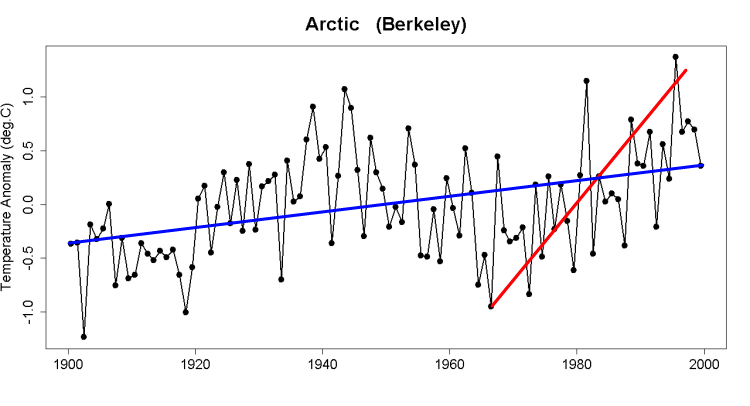
\includegraphics[scale=0.3]{images/kioto.png}
\end{center}

\end{frame}

\begin{frame}{Постановка задачи}

Пусть дан набор объектов $\mathcal{D} = \{(\mathbf{x}_i, y_i)\},
\; \mathbf{x}_i \in \mathcal{X},
\; y_i \in \mathcal{Y},
\; i \in 1, \ldots, N$, полученный из неизвестной закономерности $y = f(\mathbf{x})$. Необходимо выбрать из семейства параметрических функций
\[
H = \{h(\mathbf{x}, \theta): \mathcal{X} \times \Theta \rightarrow \mathcal{Y} \}
\]
такую $h^*(\mathbf{x}) = h(\mathbf{x}, \theta^*)$, которая наиболее точно апроксимирует $f(\mathbf{x})$.

\vspace{1em}
Задачи
\begin{itemize}
\item Классификация: $|\mathcal{Y}| < C$
\item Регрессия: $\mathcal{Y} = [a, b] \subset \mathbb{R}$
\end{itemize}

\end{frame}

\begin{frame}{Как решать}

\begin{enumerate}

\item[M] Выдвигаем гипотезу насчет {\bf модели} - семейства параметрических функций вида
\[
H = \{h(\mathbf{x}, \theta): \mathcal{X} \times \Theta \rightarrow \mathcal{Y} \},
\]
которая могла бы решить нашу задачу (model selection)

\item[L] Выбираем наилучшие параметры модели $\theta^*$, используя {\bf алгоритм обучения}
\[
A(X, Y) : (\mathcal{X}, \mathcal{Y})^N \rightarrow \Theta
\]
(learning/inference)

\item[D] Используя полученную модель $h^*(\mathbf{x}) = h(\mathbf{x}, \theta^*)$, классифицируем неизвестные объекты (decision making)

\end{enumerate}

\end{frame}

% ========================================
\section{Подходы к моделированию}
% ========================================

\begin{frame}{}

\begin{center}
\Large Подходы к моделированию
\end{center}

\end{frame}

\begin{frame}{Виды моделей}

{\bf Генеративные модели.} Смоделировать $p(\mathbf{x} | y_k)$ и $p(y_k)$, применить теорему Байеса
\[
p(y_k | \mathbf{x}) = \frac{p(\mathbf{x} | y_k) p(y_k)}{p(\mathbf{x})}
\]
и использовать $p(y_k | \mathbf{x})$ для принятия решения \\ (NB, Bayes Networks, MRF)
\vspace{1em}

{\bf Дискриминативные модели.} Смоделировать $p(y_k | \mathbf{x})$ и использовать ее для принятия решения \\ (Logistic Regression, Decision Trees)
\vspace{1em}

{\bf Функции решения.} Смоделировать напрямую $h^*(\mathbf{x}): \mathcal{X} \rightarrow \mathcal{Y}$ \\ (Linear Models, Neural Networks)

\end{frame}

\begin{frame}{Вероятностные модели VS Функции решения}

\begin{itemize}
\item[\color{green}\ding{108}] Отказ от классификации (reject option)
\item[\color{green}\ding{108}] Дисбаланс в выборке
\item[\color{green}\ding{108}] Ансамбли моделей
\item[\color{red}\ding{108}] Сильные предположения о природе данных
\item[\color{red}\ding{108}] Излишняя (вычислительная) сложность
\end{itemize}

\end{frame}

\begin{frame}{Байесовский подход к моделированию}

{\bf Идея.} Вместо фиксированного, но неизвестного $\theta^*$ ищем апостериорное распределение $p(\theta | \mathcal{D})$\\ 
{\bf Дано.} $p(y_i)$, $p(\theta)$, $p(\mathbf{x} | \theta)$ 
\[
p(y_i | \mathbf{x}, \mathcal{D})= \frac{p(\mathbf{x} | y_i, \mathcal{D}) p(y_i | \mathcal{D})}{\sum_jp(\mathbf{x} | y_j, \mathcal{D}) p(y_j | \mathcal{D})} = \frac{p(\mathbf{x} | y_i, \mathcal{D}) p(y_i)}{\sum_jp(\mathbf{x} | y_j, \mathcal{D}) p(y_j)}
\]
Разделяем выборку по классам
\[
p(\mathbf{x} | \mathcal{D}) = \int p(\mathbf{x} | \theta) p(\theta | \mathcal{D}) d\theta
\]
Апостериорное распределение
\[
p(\theta | \mathcal{D}) = \frac{p(\mathcal{D} | \theta) p(\theta)}{\int p(\mathcal{D} | \theta) p(\theta) d\theta} = \frac{\prod_n p(\mathbf{x}_n | \theta) p(\theta)}{\int \prod_n p(\mathbf{x}_n | \theta) p(\theta) d\theta}
\]

\end{frame}

\begin{frame}{Обучение модели}

\begin{quote}
\[
LEARNING = representation + evaluation + optimization
\]
\hfill Pedro Domingos
\end{quote}

Evaluation -- критерий, который оптимизируем
\begin{itemize}
\item эмпирический риск $\rightarrow \min$
\item KL-дивергенция $\rightarrow \min$
\item функция правдоподобия $\rightarrow \max$
\item information gain $\rightarrow \max$
\end{itemize}
Optimization -- как оптимизируем
\begin{itemize}
\item unconstrained (GD, Newton+)
\item constrained (linear programming, quadratic programming)
\end{itemize}

\end{frame}

\begin{frame}{Эмпирический риск}

{\bf Функция потерь} $\mathcal{L}(\mathbf{x}, y, \theta)$ - ошибка, которую для данного $\mathbf{x}$ дает модель $h(\mathbf{x}, \theta)$ по сравнению с реальным значением $y$
\vspace{1em}

{\bf Эмпирический риск} -- средняя ошибка на обучающей выборке
\[
Q(X, Y, \theta) = \frac{1}{N} \sum_{n=1}^N \mathcal{L}(\mathbf{x}_n, y_n, \theta)
\]
\vspace{1em}

{\bf Задача} -- найти значение $\theta^*$, минимизирующее эмпирический риск
\[
\theta^* = \theta^*(X, Y) = \text{argmin}_\theta Q(X, Y, \theta)
\]

\end{frame}

\begin{frame}{Некоторые функции потерь}

\begin{itemize}
\item Индикатор ошибки
\[
\mathcal{L}(\mathbf{x}, y, \theta) = 0 \text{\;if\;} h(\mathbf{x}, \theta) = y \text{\;else\;} 1
\]
\item Функция Минковского 
\[
\mathcal{L}(\mathbf{x}, y, \theta) = |y - h(\mathbf{x}, \theta)|^q
\]
Частные случаи: квадратичная $q = 2$, абсолютная ошибка $q = 1$
\item Hinge
\[
\mathcal{L}(\mathbf{x}, y, \theta) = \max(0, 1 - y \times h(\mathbf{x}, \theta))
\]
\item Информационная
\[
\mathcal{L}(\mathbf{x}, y, \theta) = - \log_2 p(y | \mathbf{x}, \theta)
\]
\begin{center}

\end{center}
\end{itemize}

\end{frame}

\begin{frame}{Проблема 1. Переобучение}

\begin{block}{Задача}
Аппроксимировать обучающую выборку полиномом $M$ степени
\end{block}

\begin{center}
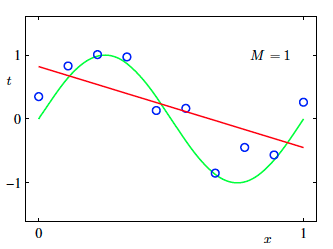
\includegraphics[scale=0.3]{images/m1.png}
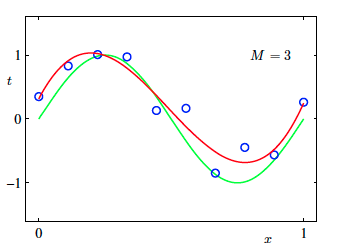
\includegraphics[scale=0.3]{images/m2.png}
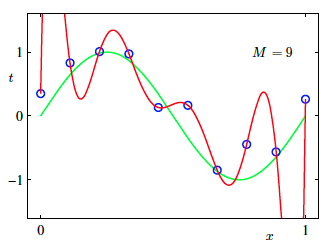
\includegraphics[scale=0.3]{images/m3.png}

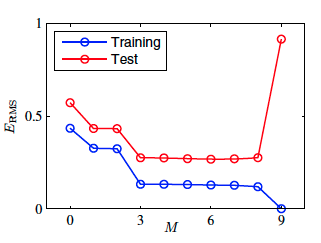
\includegraphics[scale=0.3]{images/of.png}
\end{center}

\end{frame}

\begin{frame}{Проблема 2. Проклятие размерности}

\begin{block}{Задача}
Классифицировать объекты.
\end{block}

\begin{center}
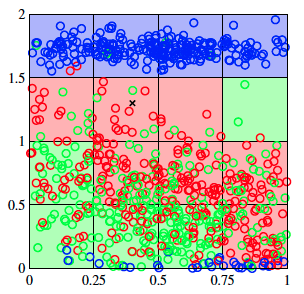
\includegraphics[scale=0.3]{images/pts.png}

\includegraphics[scale=0.4]{images/curse.png}
\end{center}

\end{frame}

% ========================================
\section{Теория принятия решений}
% ========================================

\begin{frame}{}

\begin{center}
\Large Теория принятия решений
\end{center}

\end{frame}

\begin{frame}{Классификация}

{\bf Пусть}

$\mathcal{R}_k$ -- область, такая что все $\mathbf{x} \in \mathcal{R}_k$ относим к $y_k$

{\bf Дано}

$R_{kj}$ -- риск, связанный с отнесением объекта класса $y_k$ к классу $y_j$

{\bf Найти}

$\forall k: \mathcal{R}_k$, такие, что математическое ожидание риска $E[R]$ минимально.

\[
E[R] = \sum_k \sum_j \int_{\mathcal{R}_j} R_{kj} p(y_k | \mathbf{x}) p(\mathbf{x}) dx
\]

\end{frame}

\begin{frame}{Медицинская диагностика}

Матрица риска $[R_{kj}]$

\begin{center}
\begin{tabular}{r | c c}
 & sick & normal \\
\hline
sick & 0 & 10 \\
normal & 1 & 0 
\end{tabular}
\end{center}

Условные вероятности $p(y_k | x)$
\[ 
p(\mathtt{normal} | \mathtt{moving}) = 0.9, \; p(\mathtt{normal} | {\mathtt{not\;moving}}) = 0.3
\]
Вероятности $p(x)$
\[
p(\mathtt{moving}) = 0.7
\]
Требуется определить $\mathcal{R}_{\mathtt{sick}}$, $\mathcal{R}_{\mathtt{normal}}$

\end{frame}

\begin{frame}{Регрессия}

Те же виды моделей: {\bf генеративные}, {\bf дискриминативные}, {\bf функция решения}
\vspace{1em}

Задана функция риска
\[
R(y, h(\mathbf{x}))
\]
Математическое ожидание $E[R]$
\[
E[R] = \int \!\! \int R(y, h(\mathbf{x})) p(\mathbf{x}, y) d\mathbf{x} dy
\]
Для квадратичной функции риска $R(y, h(\mathbf{x})) = [y - h(\mathbf{x})]^2$
\[
h(x) = E_y[h | \mathbf{x}] = \int y p(y | \mathbf{x}) dy
\]

\end{frame}

% ========================================
\section{Оценка результатов классификации}
% ========================================

\begin{frame}{}

\begin{center}
\Large Оценка результатов классификации
\end{center}

\end{frame}

\begin{frame}{Как оценить различные модели?}

\begin{block}{Идея}
использовать долю неверно классифицированных объектов \\ (error rate)
\end{block}

\begin{alertblock}{Важное замечание}
error rate на обучающей выборке {\bf НЕ} является хорошим показателем качества модели
\end{alertblock}

\end{frame}

\begin{frame}{Решение 1: разделение выборки}

Делим обучающую выборку на {\bf тренировочную}, {\bf валидационную} и {\bf тестовую}

\begin{center}
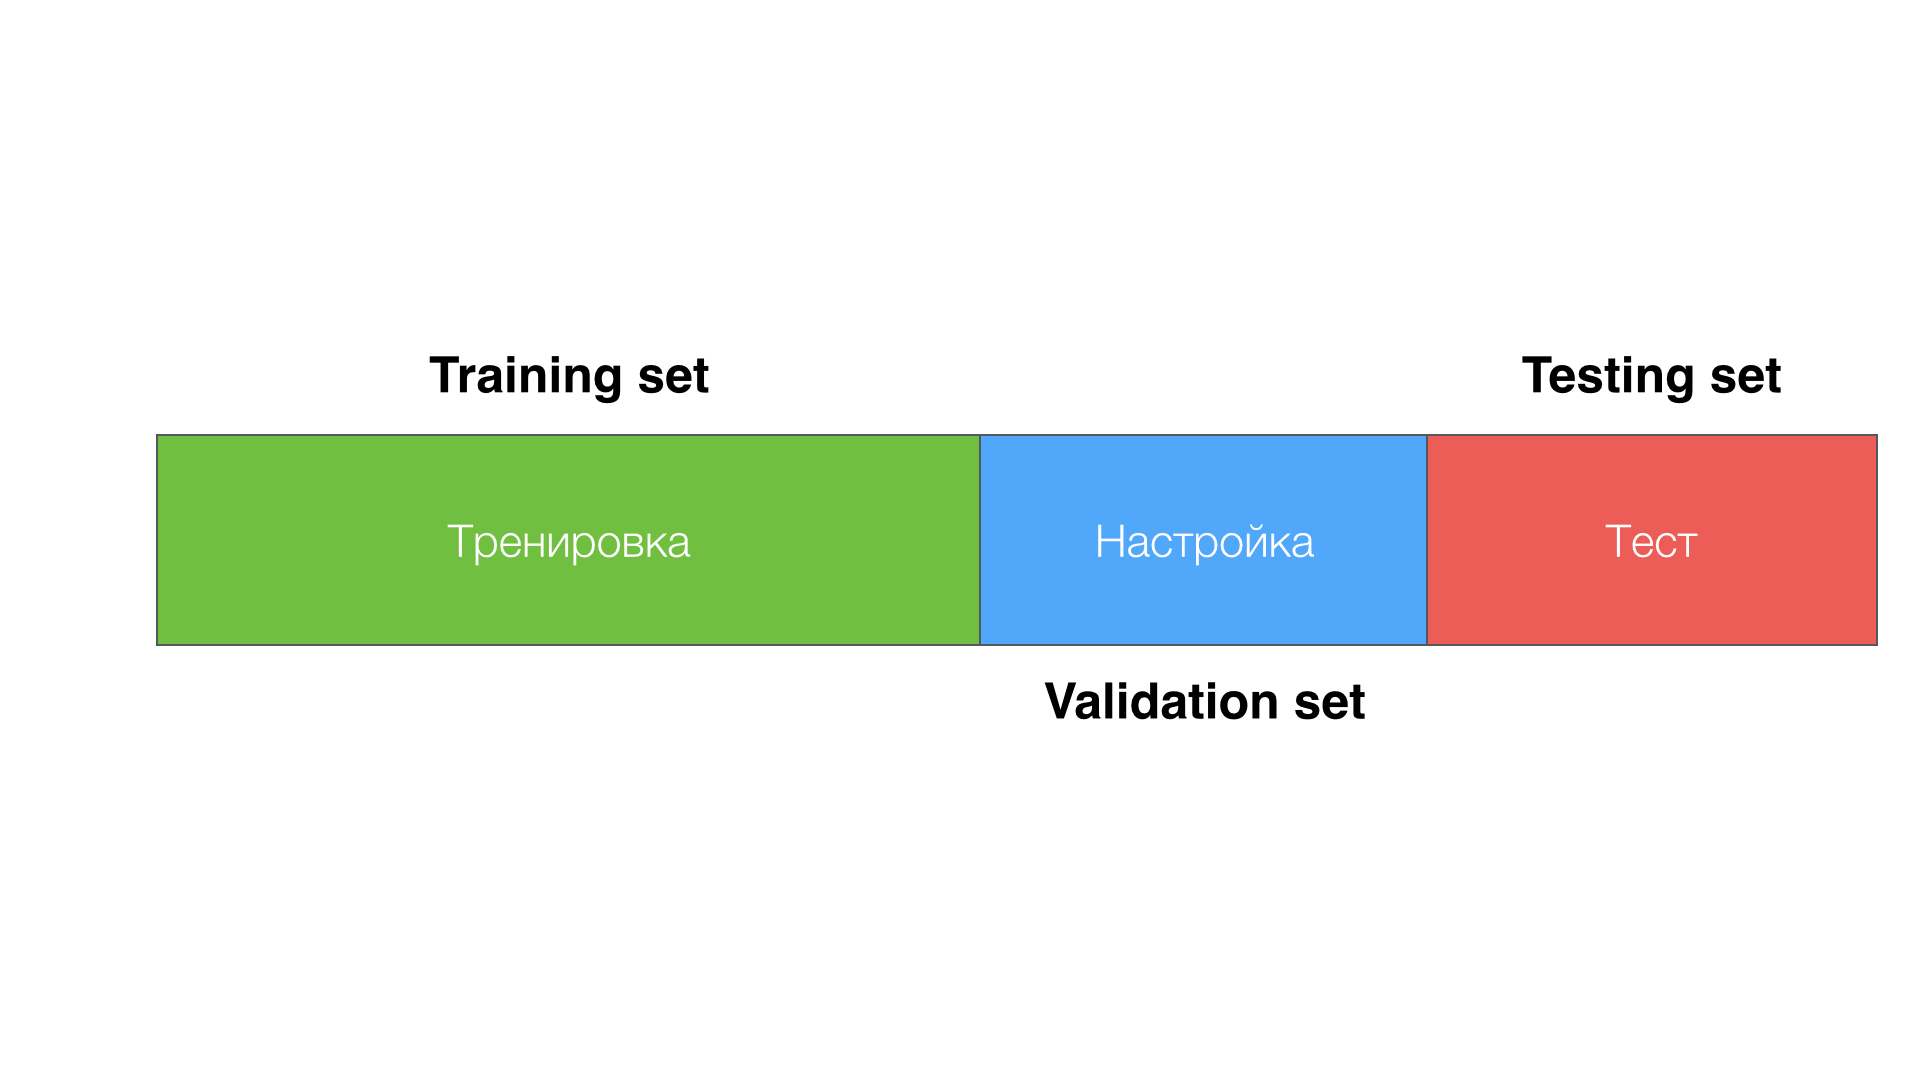
\includegraphics[scale=0.15]{images/vtt.png}
\end{center}
  
\end{frame}

\begin{frame}{Решение 2: скользящий контроль}

(n-times) (stratified) cross-validation

\begin{center}
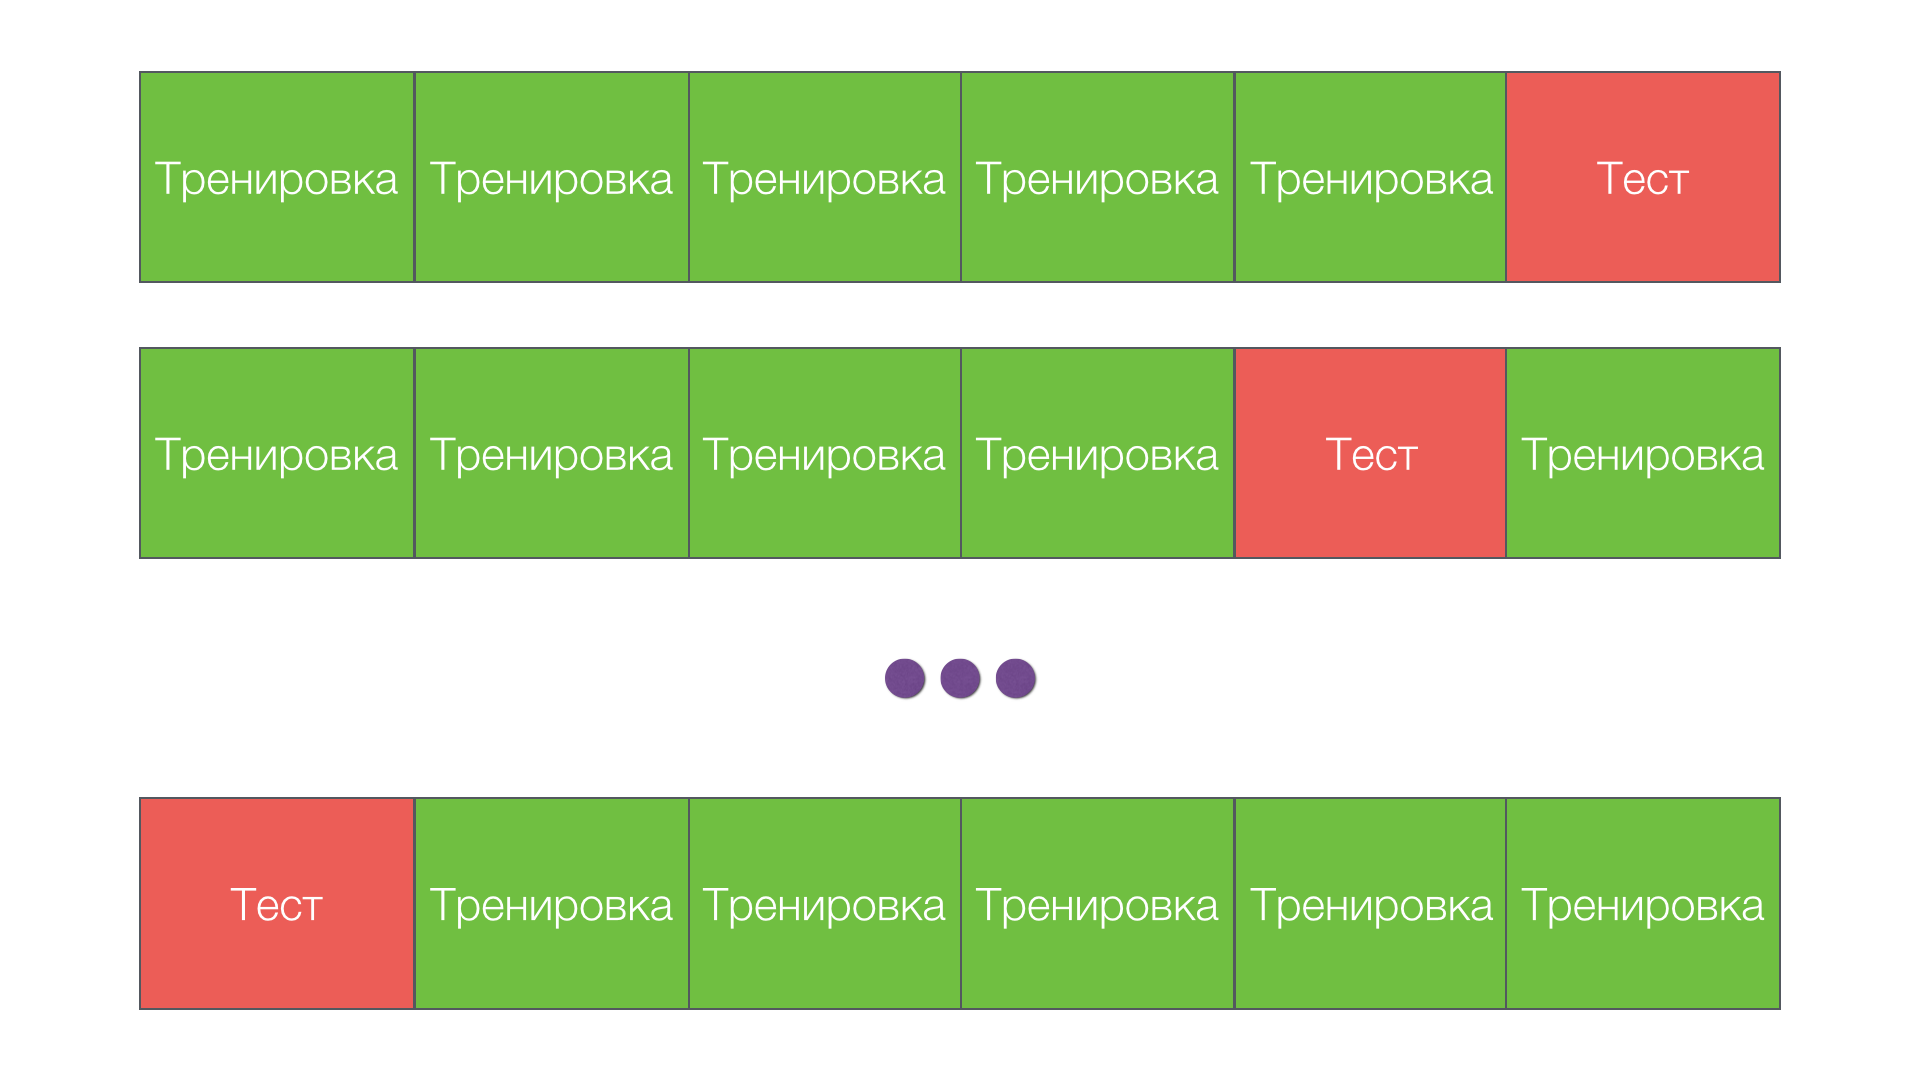
\includegraphics[scale=0.15]{images/cv.png}
\end{center}

частный случай: leave-one-out
  
\end{frame}

\begin{frame}{Решение 3: bootstrap}

выбираем в тренировочную выбоку $n$ объектов с возвращением

\begin{center}
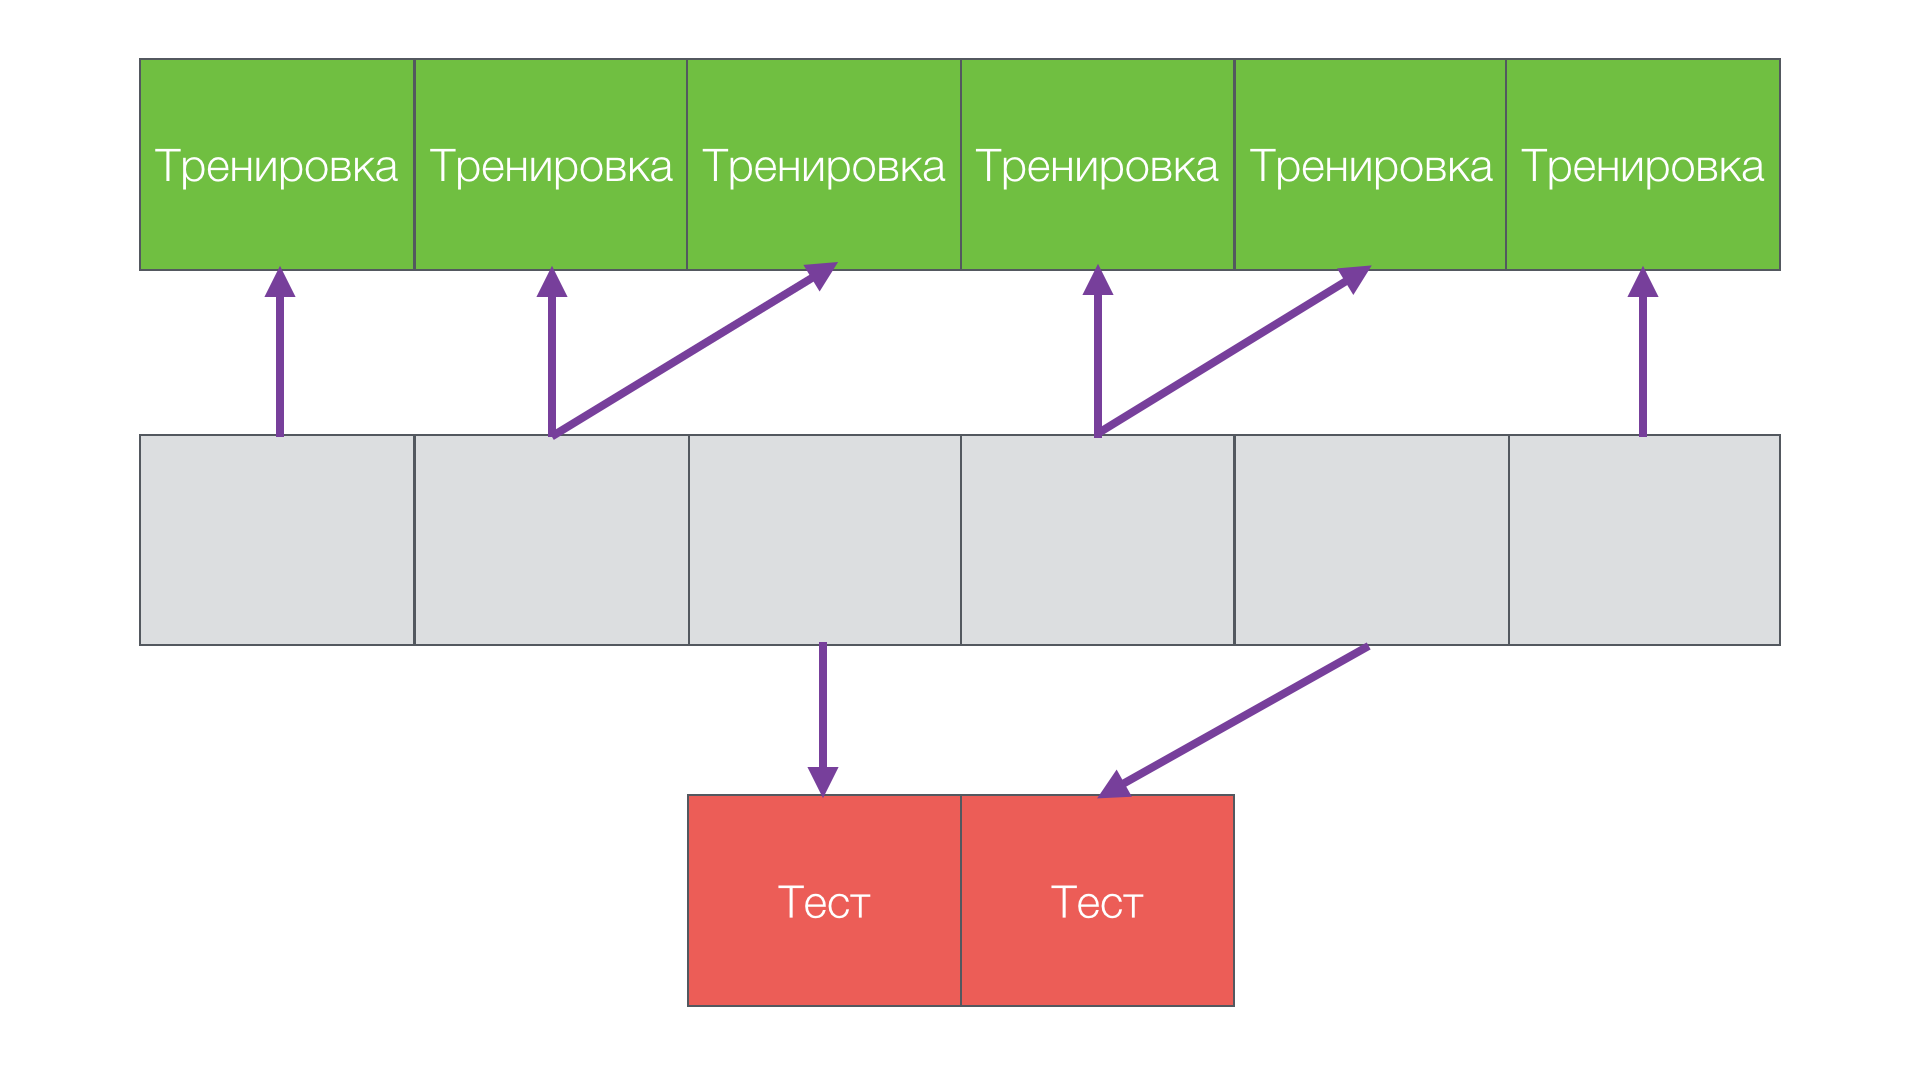
\includegraphics[scale=0.15]{images/boot.png}
\end{center}

упражнение: найти математическое ожидание размера тестовой выборки.
  
\end{frame}

\begin{frame}{Доверительный интервал для success rate}

При тестировании на $N=100$ объектах было получено $25$ ошибок. Таким образом измеренная вероятность успеха (success rate) составила $f=0.75$. Найти доверительный интервал для действительной вероятности успеха c уровнем доверия $\alpha=0.8$. 

\begin{exampleblock}{Решение}
Пусть $p$ -- действительная вероятность успеха в испытаниях бернулли, тогда
\[
f \sim \mathcal{N}\left( p, p(1-p)/N \right).
\]
Воспользовавшись табличным значением $P(-z \leq \mathcal{N}(0,1) \leq z) = \alpha$, имеем
\[
P\left(-z \leq \frac{f-p}{\sqrt{p(1-p)/N}} \leq z \right) = \alpha,
\]
откуда
\[
p \in \left(f + \frac{z^2}{2N} \pm z \sqrt{\frac f N - \frac{f^2}{N}+\frac{z^2}{4N^2}} \right)/\left(1 + \frac {z^2}{N} \right) = [0.69, 0.80]
\]
\end{exampleblock}
  
\end{frame}

\begin{frame}{Метрики качества. Вероятностные модели.}

Пусть $y_i$ - действительный класс для объекта $\mathbf{x}_i$
\begin{itemize}
\item  Information loss 
\[
- \frac 1 N \sum_i \log_2 p(y_i | \mathbf{x}_i)
\]
\item Quadratic loss 
\[
\frac 1 N \sum_j (p(y_j | \mathbf{x}_i) - a_j(\mathbf{x}_i))^2,
\] 
где
\[
a_j(\mathbf{x}_i) = \begin{cases}
1, \;\text{если}\;C_j = y_i\\
0, \;\text{иначе}
\end{cases} 
\]
\end{itemize}

\end{frame}

\begin{frame}{Метрики качества. Функции решения.}

\begin{center}
\begin{tabular}{|c r | c c|}
\cline{3-4}
 \multicolumn{2}{c|}{} & \multicolumn{2}{c|}{Предсказанный} \\
 \cline{3-4}
 \multicolumn{2}{c|}{} & {\bf true} & {\bf false} \\
 \hline
 \multirow{2}{*}{Действительный} & \multicolumn{1}{|c|}{\bf true} & TP & FN \\
 & \multicolumn{1}{|c|}{\bf false}  & FP & TN \\
 \hline
\end{tabular}
\end{center}

\[
success\;rate = accuracy = \frac{TP + TN}{TP + FP + FN + TN}
\]
\[
recall = TPR = \frac{TP}{TP + FN};\;\;precision = \frac{TP}{TP + FP}
\]
\[
FPR = \frac{FP}{FP + TN}
\]
\[
affinity = lift = \frac{accuracy}{p}
\]

\end{frame}

\begin{frame}{Receiver Operating Characteristic}

\[
TPR = \frac{TP}{TP + FN};\;\;FPR = \frac{FP}{FP + TN}
\]

\begin{center}
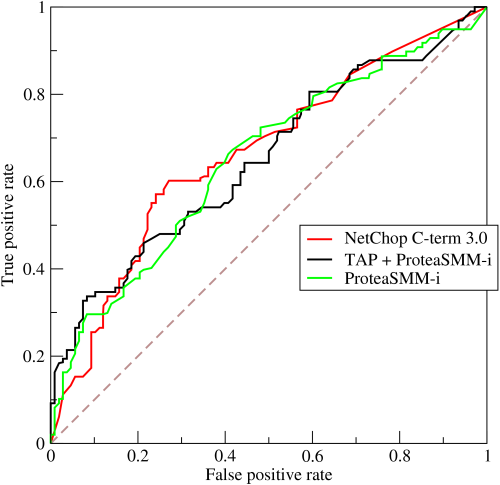
\includegraphics[scale=2.0]{images/roc.png}
\end{center}

\end{frame}

\begin{frame}{Упражнение}

\begin{exampleblock}{Простые классификаторы}
В генеральной совокупности существуют объекты 3 классов, вероятность появления которых $p_1 < p_2 < p_3$. Первый классификатор относит все объекты к классу с большей вероятностью (то есть к третьему). Второй классификатор случайно относит объект к одному из классов в соответствии с базовым распределением. Рассчитать precision и recall, которые эти классификаторы дают для каждого из 3 классов.
\end{exampleblock}

\end{frame}

\begin{frame}{Метрики качества. Регрессия}

\[
MSE = \frac 1 N \sum (h(\mathbf{x}_i) - y_i)^2, \;\; RMSE = \sqrt{MSE}
\]
\[
MAE =  \frac 1 N \sum |h(\mathbf{x}_i) - y_i|, \;\; RMAE = \sqrt{MAE}
\]
\[
RSE =  \frac{\sum (h(\mathbf{x}_i) - y_i)^2}{\sum (y_i - \bar{y})^2}
\]
\[
correlation = \frac{S_{hy}}{\sqrt{S_h S_y}};\;\; S_{yh} = \frac{\sum(h(i)-\overline{h(i)})(y_i - \bar y)}{N-1}
\]
\[
S_{h} = \frac{\sum(h(i)-\overline{h(i)})^2}{N-1};\;\;S_{y} = \frac{\sum(y_i - \bar y)^2}{N-1}
\]

\end{frame}

\begin{frame}{NFLT, MDL, AIC и все такое}

\begin{block}{No free lunch theorem}
Не существует единственной лучшей модели, решающей все задачи
\end{block}

\begin{block}{Minimum description length}
Лучшая гипотеза о данных -- та, которая ведет к самому краткому их описанию
\end{block}
\begin{block}{Akaike information criterion (AIC)}
\[
model = \arg\max	\ln p(\mathcal{D} | \theta_{ML}) - \|\theta\|
\]
\end{block}

\end{frame}

\begin{frame}[plain]
\begin{center}
{\Large Вопросы}
\end{center}
\end{frame}

\end{document}